\documentclass[11pt,a4paper]{article}

% Packages
\usepackage[utf8]{inputenc}
\usepackage[T1]{fontenc}
\usepackage{amsmath,amssymb}
\usepackage{graphicx}
\usepackage{booktabs}
\usepackage{array}
\usepackage{multirow}
\usepackage{xcolor}
\usepackage{hyperref}
\usepackage{geometry}
\usepackage{float}
\usepackage{algorithm}
\usepackage{algpseudocode}
\usepackage{listings}
\usepackage{caption}
\usepackage{subcaption}
\usepackage{tikz}
\usetikzlibrary{shapes,arrows,positioning,fit,backgrounds}

% Page geometry
\geometry{margin=1in}

% Colors
\definecolor{codeblue}{rgb}{0.13,0.53,0.79}
\definecolor{codegray}{rgb}{0.5,0.5,0.5}
\definecolor{codegreen}{rgb}{0.0,0.5,0.0}

% Hyperref setup
\hypersetup{
    colorlinks=true,
    linkcolor=blue,
    filecolor=magenta,
    urlcolor=cyan,
    citecolor=blue
}

% Code listing style
\lstset{
    basicstyle=\ttfamily\small,
    keywordstyle=\color{codeblue},
    commentstyle=\color{codegray},
    stringstyle=\color{codegreen},
    numbers=left,
    numberstyle=\tiny\color{codegray},
    frame=single,
    breaklines=true,
    captionpos=b
}

% Title
\title{
    \vspace{-1cm}
    \textbf{SYNAPSE 2026} \\
    \large Surface Electromyography Gesture Classification \\
    Using Hybrid Deep Learning \\
    \vspace{0.5cm}
    \normalsize PARSEC 6.0 Neurotech Challenge | IIT Dharwad
}

\author{Team Amrut Ra}
\date{January 2026}

\begin{document}

\maketitle

\begin{abstract}
This report presents our solution for the PARSEC 6.0 Neurotech Challenge: a surface electromyography (sEMG) gesture classification system using hybrid deep learning. Our approach combines convolutional neural networks with recurrent architectures and hand-crafted features to classify 5 distinct hand gestures from 8-channel EMG signals. The model achieves \textbf{74.29\% $\pm$ 3.15\%} accuracy with only \textbf{45,781 parameters}, demonstrating that lightweight architectures can achieve competitive performance on neurophysiological signal classification tasks. Key innovations include multi-scale temporal convolutions, channel attention mechanisms, bidirectional GRU with temporal attention, and strategic data augmentation for class imbalance handling.
\end{abstract}

\tableofcontents
\newpage

% ============================================================================
\section{Introduction}
% ============================================================================

\subsection{Problem Statement}

Surface electromyography (sEMG) provides a non-invasive method to measure electrical activity produced by skeletal muscles. In human-computer interaction and prosthetics, sEMG-based gesture recognition enables intuitive control interfaces. However, classifying gestures from EMG signals presents several challenges:

\begin{itemize}
    \item \textbf{High inter-subject variability}: EMG patterns vary significantly across individuals due to anatomical differences, electrode placement, and muscle activation patterns.
    \item \textbf{Temporal dynamics}: Gestures involve complex temporal patterns that evolve over time.
    \item \textbf{Noise susceptibility}: EMG signals are contaminated by powerline interference, motion artifacts, and electrode noise.
    \item \textbf{Class imbalance}: Certain gestures may exhibit similar activation patterns, leading to confusion.
\end{itemize}

\subsection{Dataset Overview}

The Synapse Dataset consists of:
\begin{itemize}
    \item \textbf{Subjects}: 25 individuals
    \item \textbf{Sessions}: 3 per subject
    \item \textbf{Gestures}: 5 classes (G0-G4)
    \item \textbf{Trials}: 7 per gesture per session
    \item \textbf{Total samples}: 2,625 (25 $\times$ 3 $\times$ 5 $\times$ 7)
    \item \textbf{Channels}: 8 EMG electrodes
    \item \textbf{Sampling rate}: 1000 Hz
\end{itemize}

\subsection{Our Contribution}

We present a hybrid deep learning architecture that:
\begin{enumerate}
    \item Combines CNN-based feature extraction with recurrent modeling
    \item Integrates 144 hand-crafted features with learned representations
    \item Employs attention mechanisms at both channel and temporal levels
    \item Maintains a lightweight parameter count ($<$50K) suitable for edge deployment
\end{enumerate}

% ============================================================================
\section{Signal Processing Pipeline}
% ============================================================================

\subsection{Raw Signal Characteristics}

EMG signals exhibit characteristics that require careful preprocessing:
\begin{itemize}
    \item Frequency content primarily in 20-450 Hz range
    \item Powerline interference at 50/60 Hz
    \item Baseline wander and DC offset
    \item High-frequency noise from electrode-skin interface
\end{itemize}

\subsection{Filtering Strategy}

Our preprocessing pipeline applies:

\subsubsection{Bandpass Filtering}
A 4th-order Butterworth bandpass filter (20-450 Hz) removes:
\begin{itemize}
    \item Low-frequency motion artifacts ($<$20 Hz)
    \item High-frequency noise ($>$450 Hz)
\end{itemize}

The transfer function is:
\begin{equation}
    H(s) = \frac{1}{\sqrt{1 + \left(\frac{s}{\omega_c}\right)^{2n}}}
\end{equation}
where $n=4$ is the filter order and $\omega_c$ represents the cutoff frequencies.

\subsubsection{Notch Filtering}
IIR notch filters at 50 Hz and 60 Hz (Q=30) remove powerline interference:
\begin{equation}
    H(z) = \frac{1 - 2\cos(\omega_0)z^{-1} + z^{-2}}{1 - 2r\cos(\omega_0)z^{-1} + r^2 z^{-2}}
\end{equation}

\subsection{Normalization}

We employ \textbf{RobustScaler} normalization which uses median and interquartile range (IQR):
\begin{equation}
    x_{norm} = \frac{x - \text{median}(x)}{\text{IQR}(x)}
\end{equation}

This approach is robust to outliers common in EMG signals.

% ============================================================================
\section{Feature Engineering}
% ============================================================================

We extract 144 hand-crafted features (18 per channel $\times$ 8 channels) capturing complementary signal characteristics.

\subsection{Time-Domain Features}

\begin{table}[H]
\centering
\caption{Time-Domain Features}
\begin{tabular}{lll}
\toprule
\textbf{Feature} & \textbf{Formula} & \textbf{Interpretation} \\
\midrule
Mean Absolute Value (MAV) & $\frac{1}{N}\sum_{i=1}^{N}|x_i|$ & Average signal amplitude \\
Root Mean Square (RMS) & $\sqrt{\frac{1}{N}\sum_{i=1}^{N}x_i^2}$ & Signal power \\
Waveform Length (WL) & $\sum_{i=1}^{N-1}|x_{i+1} - x_i|$ & Signal complexity \\
Zero Crossings (ZC) & $\sum_{i=1}^{N-1}\mathbb{1}[x_i \cdot x_{i+1} < 0]$ & Frequency estimate \\
Slope Sign Changes (SSC) & $\sum_{i=2}^{N-1}\mathbb{1}[(x_i - x_{i-1})(x_i - x_{i+1}) > 0]$ & High-freq content \\
Variance (VAR) & $\frac{1}{N}\sum_{i=1}^{N}(x_i - \bar{x})^2$ & Signal variability \\
Integrated EMG (IEMG) & $\sum_{i=1}^{N}|x_i|$ & Total signal energy \\
Willison Amplitude (WAMP) & $\sum_{i=1}^{N-1}\mathbb{1}[|x_{i+1} - x_i| > \theta]$ & Motor unit activity \\
Log Detector & $\exp\left(\frac{1}{N}\sum_{i=1}^{N}\log|x_i|\right)$ & Geometric mean \\
\bottomrule
\end{tabular}
\end{table}

\subsection{Hjorth Parameters}

Hjorth parameters characterize signal dynamics:
\begin{align}
    \text{Activity} &= \text{Var}(x) \\
    \text{Mobility} &= \sqrt{\frac{\text{Var}(x')}{\text{Var}(x)}} \\
    \text{Complexity} &= \frac{\text{Mobility}(x')}{\text{Mobility}(x)}
\end{align}

\subsection{Spectral Features}

Using Welch's method for power spectral density estimation:

\begin{itemize}
    \item \textbf{Mean Frequency}: $f_{mean} = \frac{\sum_i f_i \cdot P_i}{\sum_i P_i}$
    \item \textbf{Median Frequency}: Frequency at 50\% cumulative power
    \item \textbf{Spectral Entropy}: $H = -\sum_i p_i \log_2 p_i$ where $p_i = P_i / \sum P$
    \item \textbf{Band Powers}: Relative power in bands [20-50], [50-100], [100-200], [200-450] Hz
\end{itemize}

\subsection{Autoregressive Coefficients}

AR(2) model coefficients capture signal predictability:
\begin{equation}
    x_t = \sum_{i=1}^{p} a_i x_{t-i} + \epsilon_t
\end{equation}

% ============================================================================
\section{Model Architecture}
% ============================================================================

\subsection{Architecture Overview}

\begin{figure}[H]
\centering
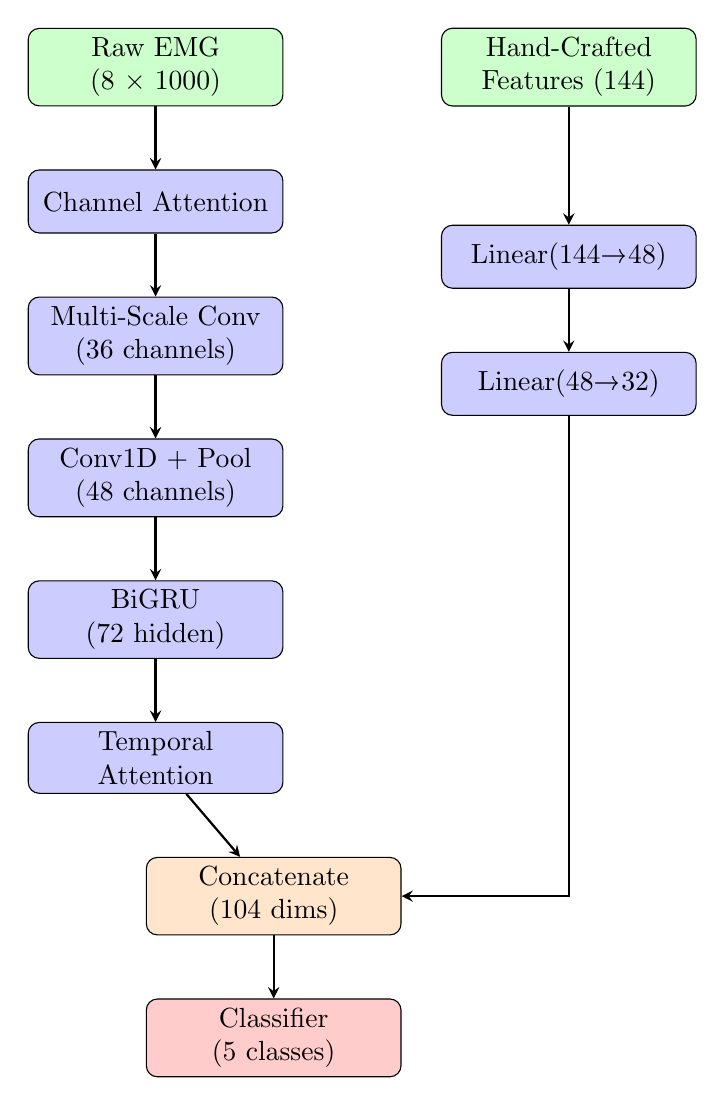
\begin{tikzpicture}[
    node distance=0.8cm,
    block/.style={rectangle, draw, fill=blue!20, text width=3cm, text centered, rounded corners, minimum height=0.8cm},
    arrow/.style={thick,->,>=stealth}
]

% Input
\node[block, fill=green!20] (input) {Raw EMG\\(8 $\times$ 1000)};
\node[block, fill=green!20, right=2cm of input] (features) {Hand-Crafted\\Features (144)};

% Signal branch
\node[block, below=of input] (attn) {Channel Attention};
\node[block, below=of attn] (msconv) {Multi-Scale Conv\\(36 channels)};
\node[block, below=of msconv] (conv2) {Conv1D + Pool\\(48 channels)};
\node[block, below=of conv2] (gru) {BiGRU\\(72 hidden)};
\node[block, below=of gru] (tempattn) {Temporal Attention};

% Feature branch
\node[block, below=1.5cm of features] (fc1) {Linear(144→48)};
\node[block, below=of fc1] (fc2) {Linear(48→32)};

% Fusion
\node[block, fill=orange!20, below=of tempattn, xshift=1.5cm] (concat) {Concatenate\\(104 dims)};

% Output
\node[block, fill=red!20, below=of concat] (classifier) {Classifier\\(5 classes)};

% Arrows
\draw[arrow] (input) -- (attn);
\draw[arrow] (attn) -- (msconv);
\draw[arrow] (msconv) -- (conv2);
\draw[arrow] (conv2) -- (gru);
\draw[arrow] (gru) -- (tempattn);
\draw[arrow] (tempattn) -- (concat);

\draw[arrow] (features) -- (fc1);
\draw[arrow] (fc1) -- (fc2);
\draw[arrow] (fc2) |- (concat);

\draw[arrow] (concat) -- (classifier);

\end{tikzpicture}
\caption{Model Architecture Overview}
\end{figure}

\subsection{Channel Attention Module}

The channel attention mechanism learns importance weights for each EMG channel:
\begin{equation}
    \alpha_c = \sigma\left(W_2 \cdot \text{ReLU}(W_1 \cdot \text{GAP}(X_c))\right)
\end{equation}
where GAP is global average pooling and $\sigma$ is the sigmoid function.

\subsection{Multi-Scale Convolution}

Three parallel convolution paths capture patterns at different temporal scales:
\begin{itemize}
    \item \textbf{Short-term} (kernel=3): Fine muscle activations
    \item \textbf{Medium-term} (kernel=7): Gesture transitions
    \item \textbf{Long-term} (kernel=15): Overall gesture patterns
\end{itemize}

Outputs are concatenated: $Y = [Y_3 \| Y_7 \| Y_{15}]$

\subsection{Bidirectional GRU with Temporal Attention}

The BiGRU models sequential dependencies:
\begin{align}
    \overrightarrow{h}_t &= \text{GRU}(x_t, \overrightarrow{h}_{t-1}) \\
    \overleftarrow{h}_t &= \text{GRU}(x_t, \overleftarrow{h}_{t+1}) \\
    h_t &= [\overrightarrow{h}_t \| \overleftarrow{h}_t]
\end{align}

Temporal attention weights relevant time steps:
\begin{align}
    e_t &= \tanh(W_h h_t) \\
    \alpha_t &= \frac{\exp(e_t)}{\sum_j \exp(e_j)} \\
    c &= \sum_t \alpha_t h_t
\end{align}

\subsection{Parameter Count}

\begin{table}[H]
\centering
\caption{Model Parameter Breakdown}
\begin{tabular}{lr}
\toprule
\textbf{Component} & \textbf{Parameters} \\
\midrule
Channel Attention & 36 \\
Multi-Scale Conv (3 paths) & 2,700 \\
Conv2 Block & 8,784 \\
BiGRU & 19,584 \\
Temporal Attention & 1,315 \\
Feature Branch & 8,528 \\
Classifier & 4,834 \\
\midrule
\textbf{Total} & \textbf{45,781} \\
\bottomrule
\end{tabular}
\end{table}

% ============================================================================
\section{Training Methodology}
% ============================================================================

\subsection{Data Augmentation}

Strategic augmentation for hard classes (G1, G2, G3):

\begin{table}[H]
\centering
\caption{Augmentation Strategy}
\begin{tabular}{lcc}
\toprule
\textbf{Augmentation} & \textbf{Hard Classes} & \textbf{Easy Classes} \\
\midrule
Gaussian Noise & $\mathcal{N}(0, 0.10)$ & $\mathcal{N}(0, 0.05)$ \\
Amplitude Scaling & [0.85, 1.15] & [0.90, 1.10] \\
Temporal Shift & $\pm$50 samples & $\pm$50 samples \\
Application Probability & 80\% & 50\% \\
\bottomrule
\end{tabular}
\end{table}

\textbf{Mixup Regularization}:
\begin{align}
    \tilde{x} &= \lambda x_i + (1-\lambda) x_j \\
    \tilde{y} &= \lambda y_i + (1-\lambda) y_j
\end{align}
with $\lambda \sim \text{Beta}(0.2, 0.2)$.

\subsection{Loss Function}

\textbf{Focal Loss} addresses class imbalance:
\begin{equation}
    \mathcal{L}_{FL} = -\sum_c w_c (1 - p_c)^\gamma \log(p_c)
\end{equation}
where $\gamma = 2.0$ and class weights $w = [1.0, 1.8, 1.2, 1.5, 1.0]$.

\subsection{Optimization}

\begin{itemize}
    \item \textbf{Optimizer}: AdamW with weight decay $2 \times 10^{-4}$
    \item \textbf{Learning Rate}: 0.0008 with cosine annealing
    \item \textbf{Warmup}: 5 epochs linear warmup
    \item \textbf{Gradient Clipping}: max\_norm = 1.0
    \item \textbf{Early Stopping}: 35 epochs patience
\end{itemize}

\subsection{Validation Strategy}

\textbf{5-Fold Subject-Grouped Cross-Validation}:
\begin{itemize}
    \item Subjects grouped to prevent data leakage
    \item 5 subjects per test fold
    \item 20 subjects for training (15\% validation split)
    \item Each subject appears in exactly one test fold
\end{itemize}

% ============================================================================
\section{Results}
% ============================================================================

\subsection{Cross-Validation Performance}

\begin{table}[H]
\centering
\caption{5-Fold Cross-Validation Results}
\begin{tabular}{ccccccc}
\toprule
\textbf{Fold} & \textbf{Accuracy} & \textbf{G0} & \textbf{G1} & \textbf{G2} & \textbf{G3} & \textbf{G4} \\
\midrule
1 & 73.33\% & 60.0\% & 76.2\% & 59.0\% & 73.3\% & 98.1\% \\
2 & 77.14\% & 77.1\% & 71.4\% & 82.9\% & 65.7\% & 88.6\% \\
3 & 78.10\% & 78.1\% & 84.8\% & 78.1\% & 68.6\% & 91.4\% \\
4 & 69.52\% & 49.5\% & 58.1\% & 51.4\% & 77.1\% & 91.4\% \\
5 & 73.33\% & 58.1\% & 72.4\% & 73.3\% & 72.4\% & 100.0\% \\
\midrule
\textbf{Mean} & \textbf{74.29\%} & 64.6\% & 72.6\% & 69.0\% & 71.4\% & 93.9\% \\
\textbf{Std} & $\pm$3.15\% & $\pm$11.3\% & $\pm$8.9\% & $\pm$14.5\% & $\pm$6.0\% & $\pm$4.4\% \\
\bottomrule
\end{tabular}
\end{table}

\subsection{Results Visualization}

Figure \ref{fig:results} shows the cross-validation results including confusion matrices and per-class accuracy analysis.

\begin{figure}[H]
\centering
\includegraphics[width=\textwidth]{cv_results_v11.png}
\caption{Cross-validation results: (top-left) Confusion matrix with absolute counts, (top-right) Normalized confusion matrix showing per-class accuracy, (bottom-left) Per-class accuracy across all 5 folds, (bottom-right) Mean accuracy per gesture class with standard deviation error bars.}
\label{fig:results}
\end{figure}

\subsection{Key Observations}

\begin{enumerate}
    \item \textbf{G4 dominates} (93.9\%): Distinct muscle activation pattern
    \item \textbf{G0 and G2 challenging}: High variance suggests inter-subject differences
    \item \textbf{Consistent G3}: Lowest variance despite moderate accuracy
    \item \textbf{Cross-fold stability}: $\pm$3.15\% standard deviation indicates robust model
\end{enumerate}

% ============================================================================
\section{Design Rationale}
% ============================================================================

\subsection{Why Hybrid Architecture?}

\begin{enumerate}
    \item \textbf{CNNs} excel at local pattern extraction but miss global context
    \item \textbf{RNNs} capture temporal dependencies but struggle with long sequences
    \item \textbf{Hand-crafted features} encode domain knowledge that networks may not learn
    \item \textbf{Combination} leverages complementary strengths
\end{enumerate}

\subsection{Why Attention Mechanisms?}

\begin{itemize}
    \item \textbf{Channel Attention}: Not all channels equally informative for all gestures
    \item \textbf{Temporal Attention}: Discriminative information concentrated in specific time windows
\end{itemize}

\subsection{Why Lightweight Architecture?}

\begin{enumerate}
    \item \textbf{Limited data}: 2,625 samples prone to overfitting with large models
    \item \textbf{Edge deployment}: Target platforms have compute constraints
    \item \textbf{Real-time inference}: Smaller models enable faster predictions
\end{enumerate}

Our experiments showed that increasing model complexity (V10: 122K params) led to \textit{worse} performance (60\% vs 74\%), confirming that simplicity is crucial for small datasets.

\subsection{Why These Specific Features?}

\begin{itemize}
    \item \textbf{Time-domain}: Computationally efficient, capture amplitude characteristics
    \item \textbf{Hjorth}: Standard in EEG/EMG analysis, describe signal dynamics
    \item \textbf{Spectral}: EMG frequency content differs across gestures
    \item \textbf{AR coefficients}: Model temporal correlations
\end{itemize}

% ============================================================================
\section{Conclusion}
% ============================================================================

We presented a lightweight hybrid deep learning system for sEMG gesture classification achieving 74.29\% accuracy with only 45,781 parameters. Key contributions include:

\begin{enumerate}
    \item Multi-scale temporal convolutions for capturing patterns at different time scales
    \item Dual attention mechanisms (channel and temporal) for focusing on informative signals
    \item Integration of 144 hand-crafted features with learned representations
    \item Strategic data augmentation targeting hard classes
\end{enumerate}

\subsection{Limitations and Future Work}

\begin{itemize}
    \item \textbf{G0/G2 confusion}: Additional discriminative features needed
    \item \textbf{Subject adaptation}: Transfer learning for new users
    \item \textbf{Real-time streaming}: Current model processes fixed windows
    \item \textbf{Hardware deployment}: Quantization and pruning for embedded systems
\end{itemize}

% ============================================================================
% References
% ============================================================================

\begin{thebibliography}{9}

\bibitem{hudgins1993}
Hudgins, B., Parker, P., \& Scott, R. N. (1993).
A new strategy for multifunction myoelectric control.
\textit{IEEE Transactions on Biomedical Engineering}, 40(1), 82-94.

\bibitem{phinyomark2012}
Phinyomark, A., Phukpattaranont, P., \& Limsakul, C. (2012).
Feature reduction and selection for EMG signal classification.
\textit{Expert Systems with Applications}, 39(8), 7420-7431.

\bibitem{atzori2016}
Atzori, M., et al. (2016).
Deep learning with convolutional neural networks applied to electromyography data.
\textit{Frontiers in Neurorobotics}, 10, 9.

\bibitem{hu2018}
Hu, J., Shen, L., \& Sun, G. (2018).
Squeeze-and-excitation networks.
\textit{CVPR}, 7132-7141.

\bibitem{lin2017}
Lin, T. Y., et al. (2017).
Focal loss for dense object detection.
\textit{ICCV}, 2980-2988.

\end{thebibliography}

\end{document}
